\documentclass[12pt, a4paper, oneside]{report}
\usepackage[ngerman]{babel}
\usepackage{graphicx}
\usepackage{mathtools}
\usepackage[citecolor=black, colorlinks=true, urlcolor=blue, linkcolor=black]{hyperref}
    \title{\textbf{Biosphären Mess- und Überwachungsgeräte -- Funktionsprinzipien und Bedienungsanleitung}}
    \author{Tjark Gaudich}
    \date{November 2021}
    
    \addtolength{\topmargin}{-2cm}
    \addtolength{\textheight}{2cm}
\begin{document}

\pagenumbering{Alph}
\begin{titlepage}
\maketitle
\thispagestyle{empty}
\end{titlepage}
\pagenumbering{arabic}

\section{Vorwort}
Das folgende Dokument soll gleichzeitig als Dokumentation und Bedienungsanleitung für die Biosphären Umweltmessgeräte ("die Geräte") dienen, die ich für den Astrobiologie Projektkurs 2021/2022 bei Herr Krobbach entwickelt habe. Damit soll eine Nutzung und Wartung dieser Geräte weit über den Zeitraum meiner Schullaufbahn hinaus ermöglicht werden. Besonderer Fokus wird deshalb auf die Kommunikation mit dem PC zum Auslesen der Messwerte gelegt, da dieser vulnerabel für Änderungen des Betriebssystems ist, doch auch alle anderen Aspekte der Geräte sollen so sehr vertieft werden, dass sie ohne großes Vorwissen verstanden und repariert werden können. Sämtliche Quelldateien sind zusammen mit dieser Dokumentation auf 
GitHub\cite{Github} frei zugänglich.
\tableofcontents
\listoffigures

\chapter{Mechanik}

Mechanisch lassen sich die Geräte in vier Komponenten unterteilen:
eine Grundplatte (in \autoref{fig:Querschnitt} Dunkelgrau), an der alle andere Teile und das Glas der Biosphäre befestigt werden, eine Platine mit Sensoren im Inneren (nicht gezeigt) und die Hauptplatine (grün) außen sowie ein Deckel (hellgrau), der die Elektronik vor Beschädigungen schützt.
\begin{figure}[h]
	\centering
	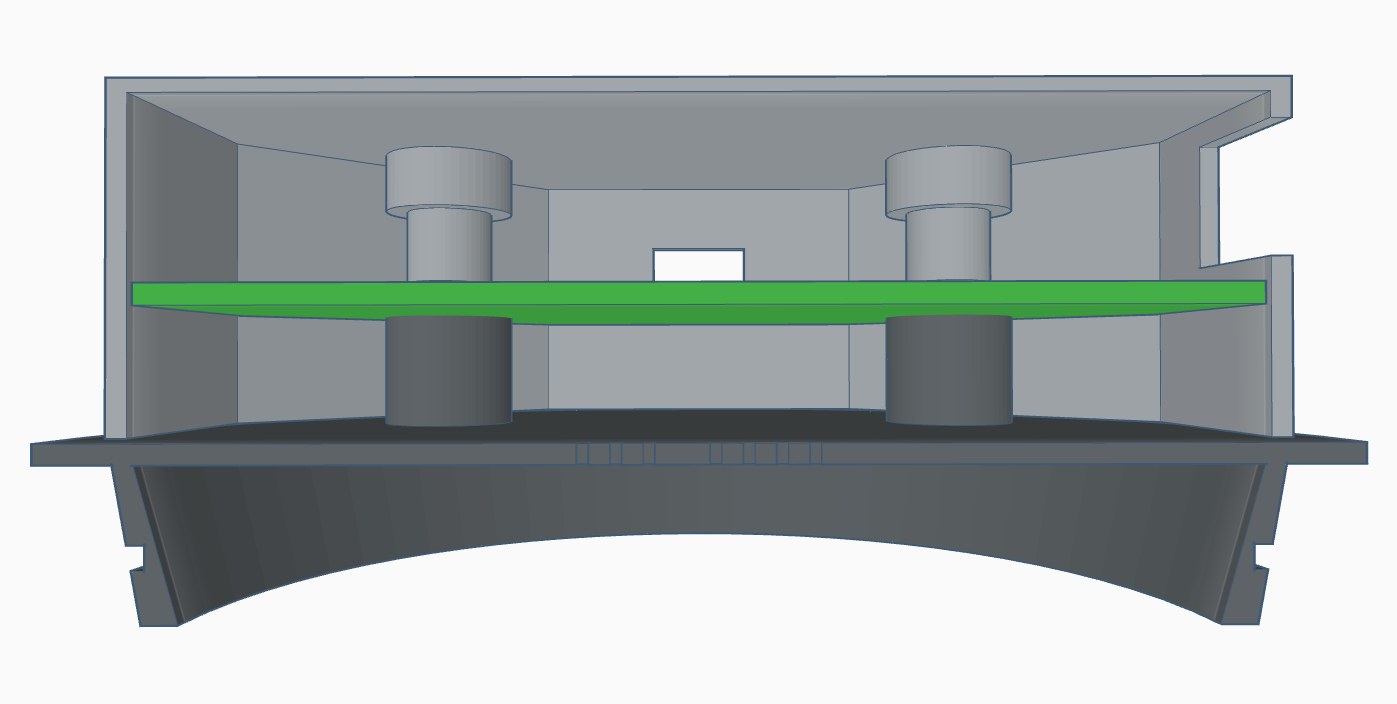
\includegraphics[width=1\textwidth]{pic/Querschnitt}
	\caption{Querschnitt durch das Gerät}
	\label{fig:Querschnitt}
\end{figure}
\\Auf die Platinen wird in \autoref{ch:elektronik} näher eingegangen, hier reicht es uns zu wissen das die unterer Platine nur über ihren Stecker befestigt wird und die obere ein Achteck von 85mm Durchmesser ist, vier Löcher mit je 50mm Abstand zueinander und 4mm Durchmesser zur Befestigung hat und 1,6mm Dick ist.

Deckel und Grundplatte sind beide aus PLA 3d gedruckt. Dabei wurde eine Auflösung von 0,2mm bei 100\% Infill verwendet
\section{Grundplatte}
Entsprechend dieser Maße ist die Oberseite der Grundplatte mit vier Röhren ausgestattet, in die M4 Einschraubmuffen montiert werden. Interessant ist jedoch die Unterseite, die in das Gurkenglas eingeklebt wird. Da die Luftmenge in der Biosphäre konstant ist kommt es bei Temperaturänderungen zu einer Druckänderung nach  dem Gesetz von Amontons \cite[S.~119]{Tafelwerk}, denen die Grundplatte und ihre Verklebung standhalten müssen. $p_0$ und $T_0$ sind dabei Druck und absolute Temperatur beim Verschließen der Biosphäre.
\begin{align}
\frac{p_0}{T_0} = \frac{p_1}{T_1} \footnote{}
\iff \Delta p = T  \times \frac{p_0}{T_0} - p_0
\label{eq:pressure}
\end{align}
Nehmen wir an, das die Biosphäre bei 20°C (293K) und Normaldruck verschlossen wurde und sich im Schlimmsten Falle auf 100°C (373K) aufgeheizt hat (darüber ist ihr Inhalt vermutlich tot, weshalb die Abdichtung irrelevant wird),
\begin{align}
\Delta p = 373K  \times \frac{1013hPa}{293K} - 1013hPa \approx 277hPa
\label{eq:pressure100C}
\end{align}
so ergibt sich nach \autoref{eq:pressure100C} ein Druckunterschied von 277hPa. Diese Druckfestigkeit mit einer Silikon Verklebung zu erreichen ist relativ einfach, beim Übergang zwischen Grundplatte und anschließendem Ring wird sie jedoch zu Herausforderung. Um eine höhere Festigkeit zu erreichen wurde dieser Übergang nach dem Druck zusätzlich mit einem Lötkolben verschmolzen. Diese Kombination hielt beim Anschließen eines Kompressors an einen Modifizierten Deckel etwa 300hPa Überdruck stand.

Falls sich zeigen sollte, das dies nicht ausreicht wäre eine Verdickung des Übergangs oder der Druck aus einem festeren Material, z.B.~Nylon, empfehlenswert.

Bei der Verklebung der Grundplatte mit dem Glas der Biosphäre sollte Aquariensilikon verwendet werden, da Sanitärsilikon für die Oranismen in der Biosphäre schädliche Zusatzstoffe enthalten kann.

\begin{figure}[h]
	\centering
	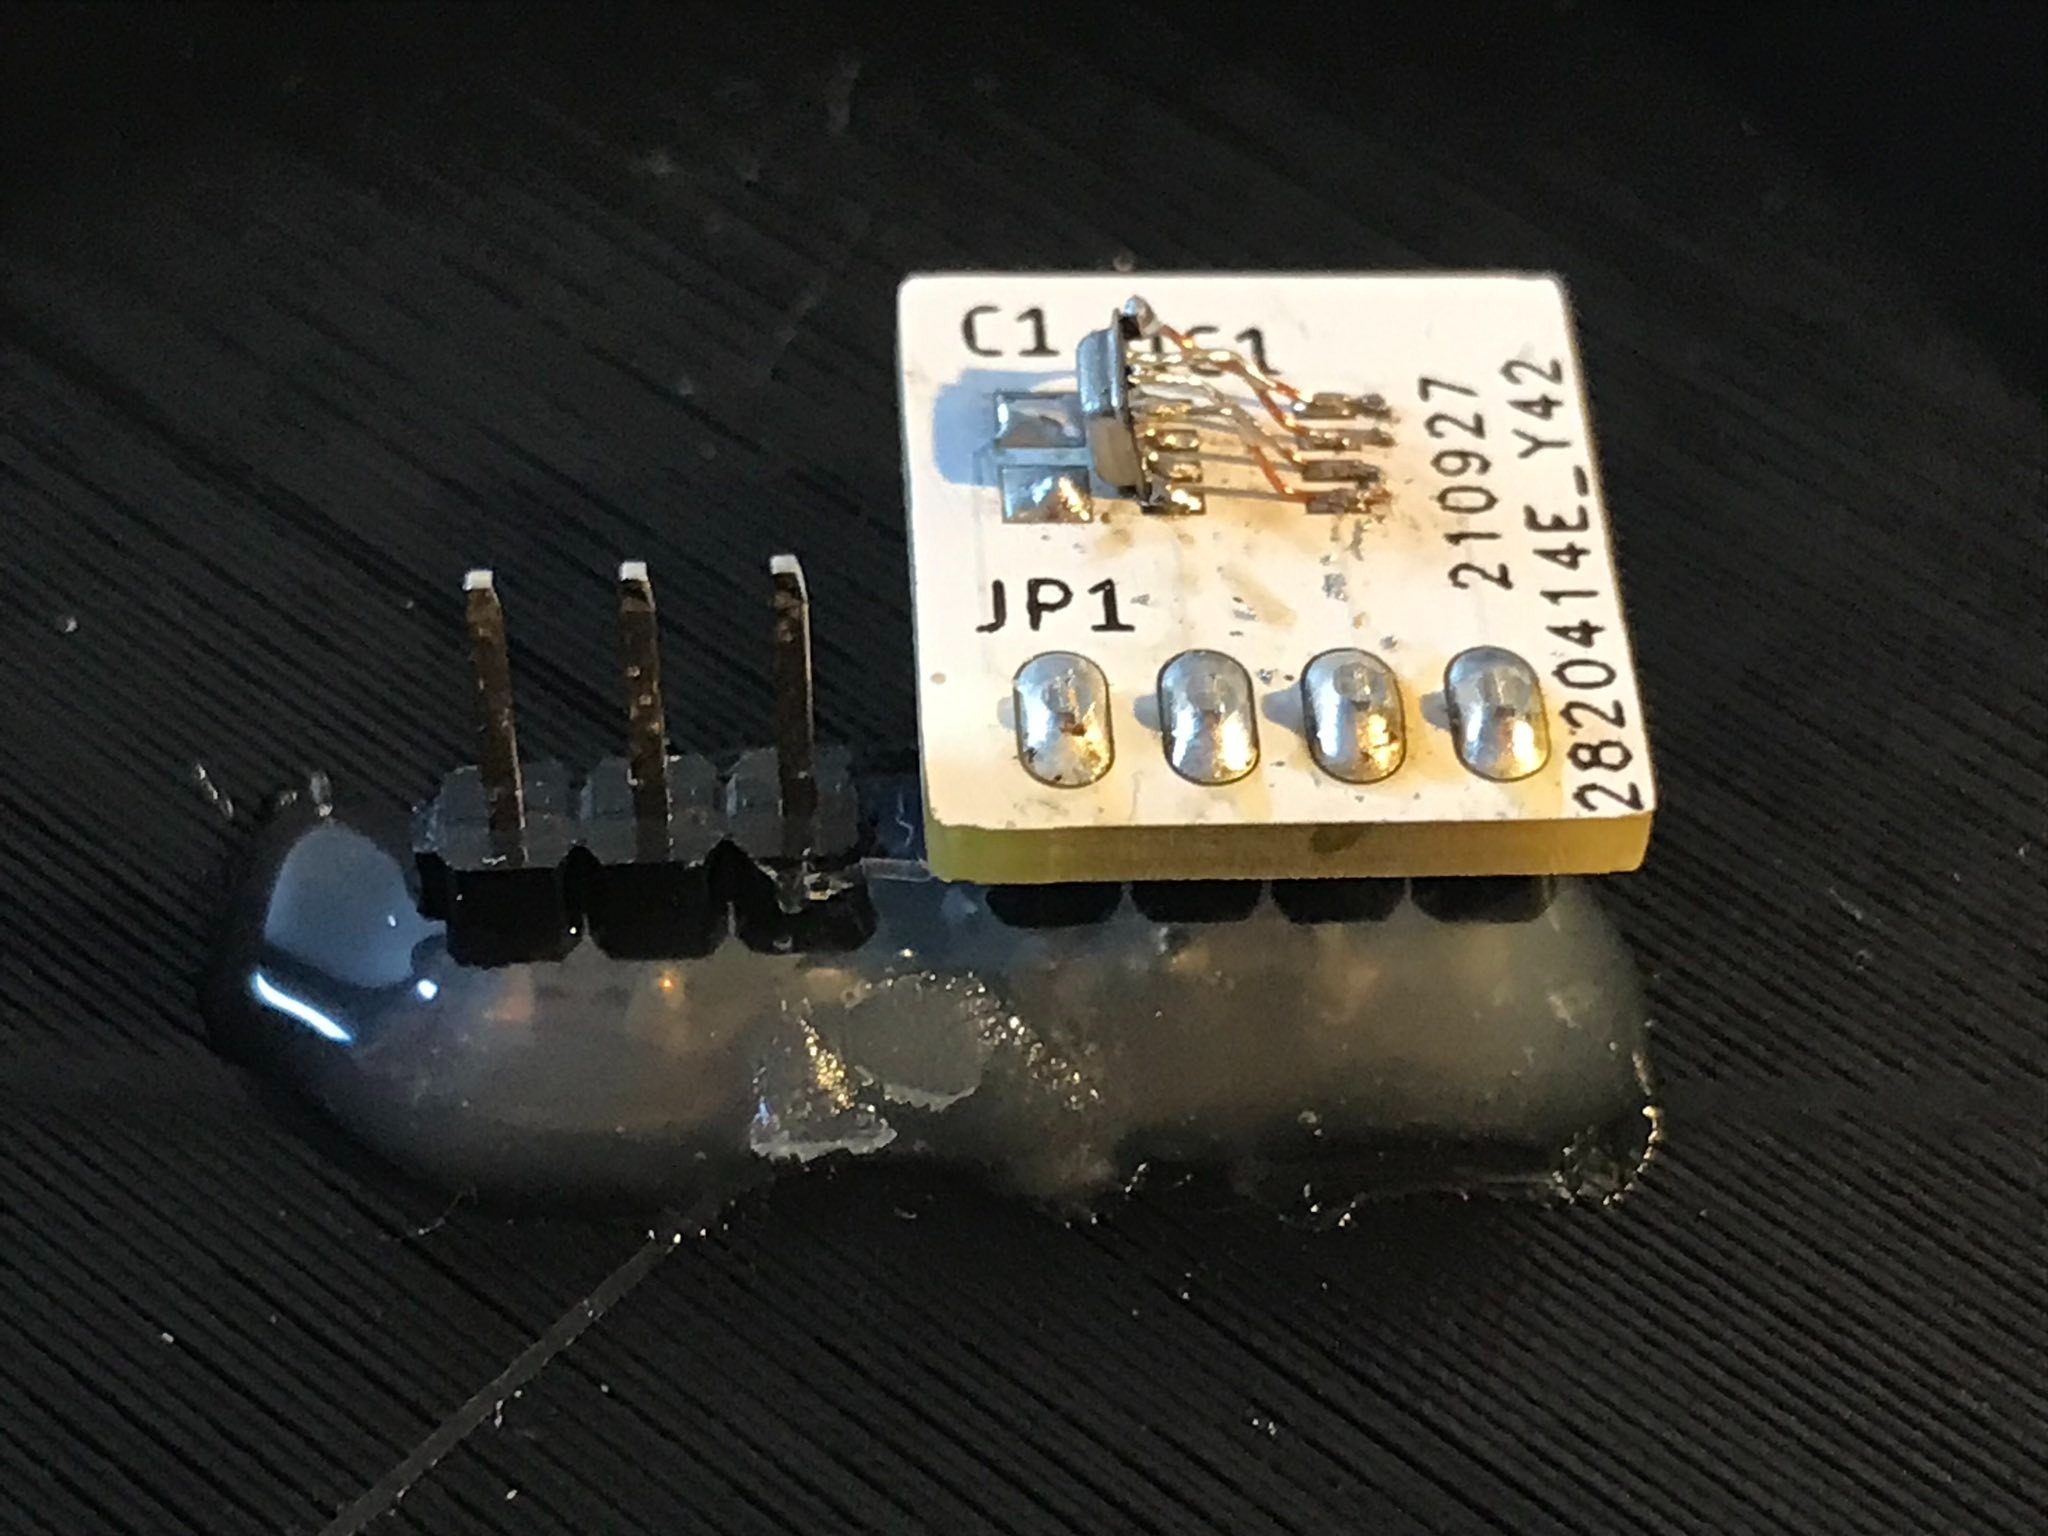
\includegraphics[height = 4cm]{pic/Stiftleisten}
	\caption{Fertig montierte Stiftleisten mit Sensorplatine}
	\label{fig:Stiftleisten}
\end{figure}

In der Platte befinden sich sieben Löcher, durch die Stiftleisten gesteckt werden um die Sensoren im Inneren mit der Hauptplatine zu verbinden. Dabei wird eine Stiftleiste von oben eingesteckt, mit Epoxidharz (UHU Endfest 3000) verklebt, von unten eine weitere Stiftleiste angelötet und die Lötstelle mit Heißkleber fixiert.

\section{Deckel}
Der Deckel besteht aus einem Achteck mit Abschlussplatte und eingesenkten Löchern, durch die er und die Hauptplatine mit vier M4~x~16 Schrauben an der Grundplatte befestigt werden. Beim Entfernen muss darauf geachtet werden, dass keine Kabel eingesteckt sind und der Deckel gerade nach oben abgezogen wird, um die durch ihn vorstehende Fotodiode nicht zu beschädigen.
\\
\begin{figure}[h]
	\centering
	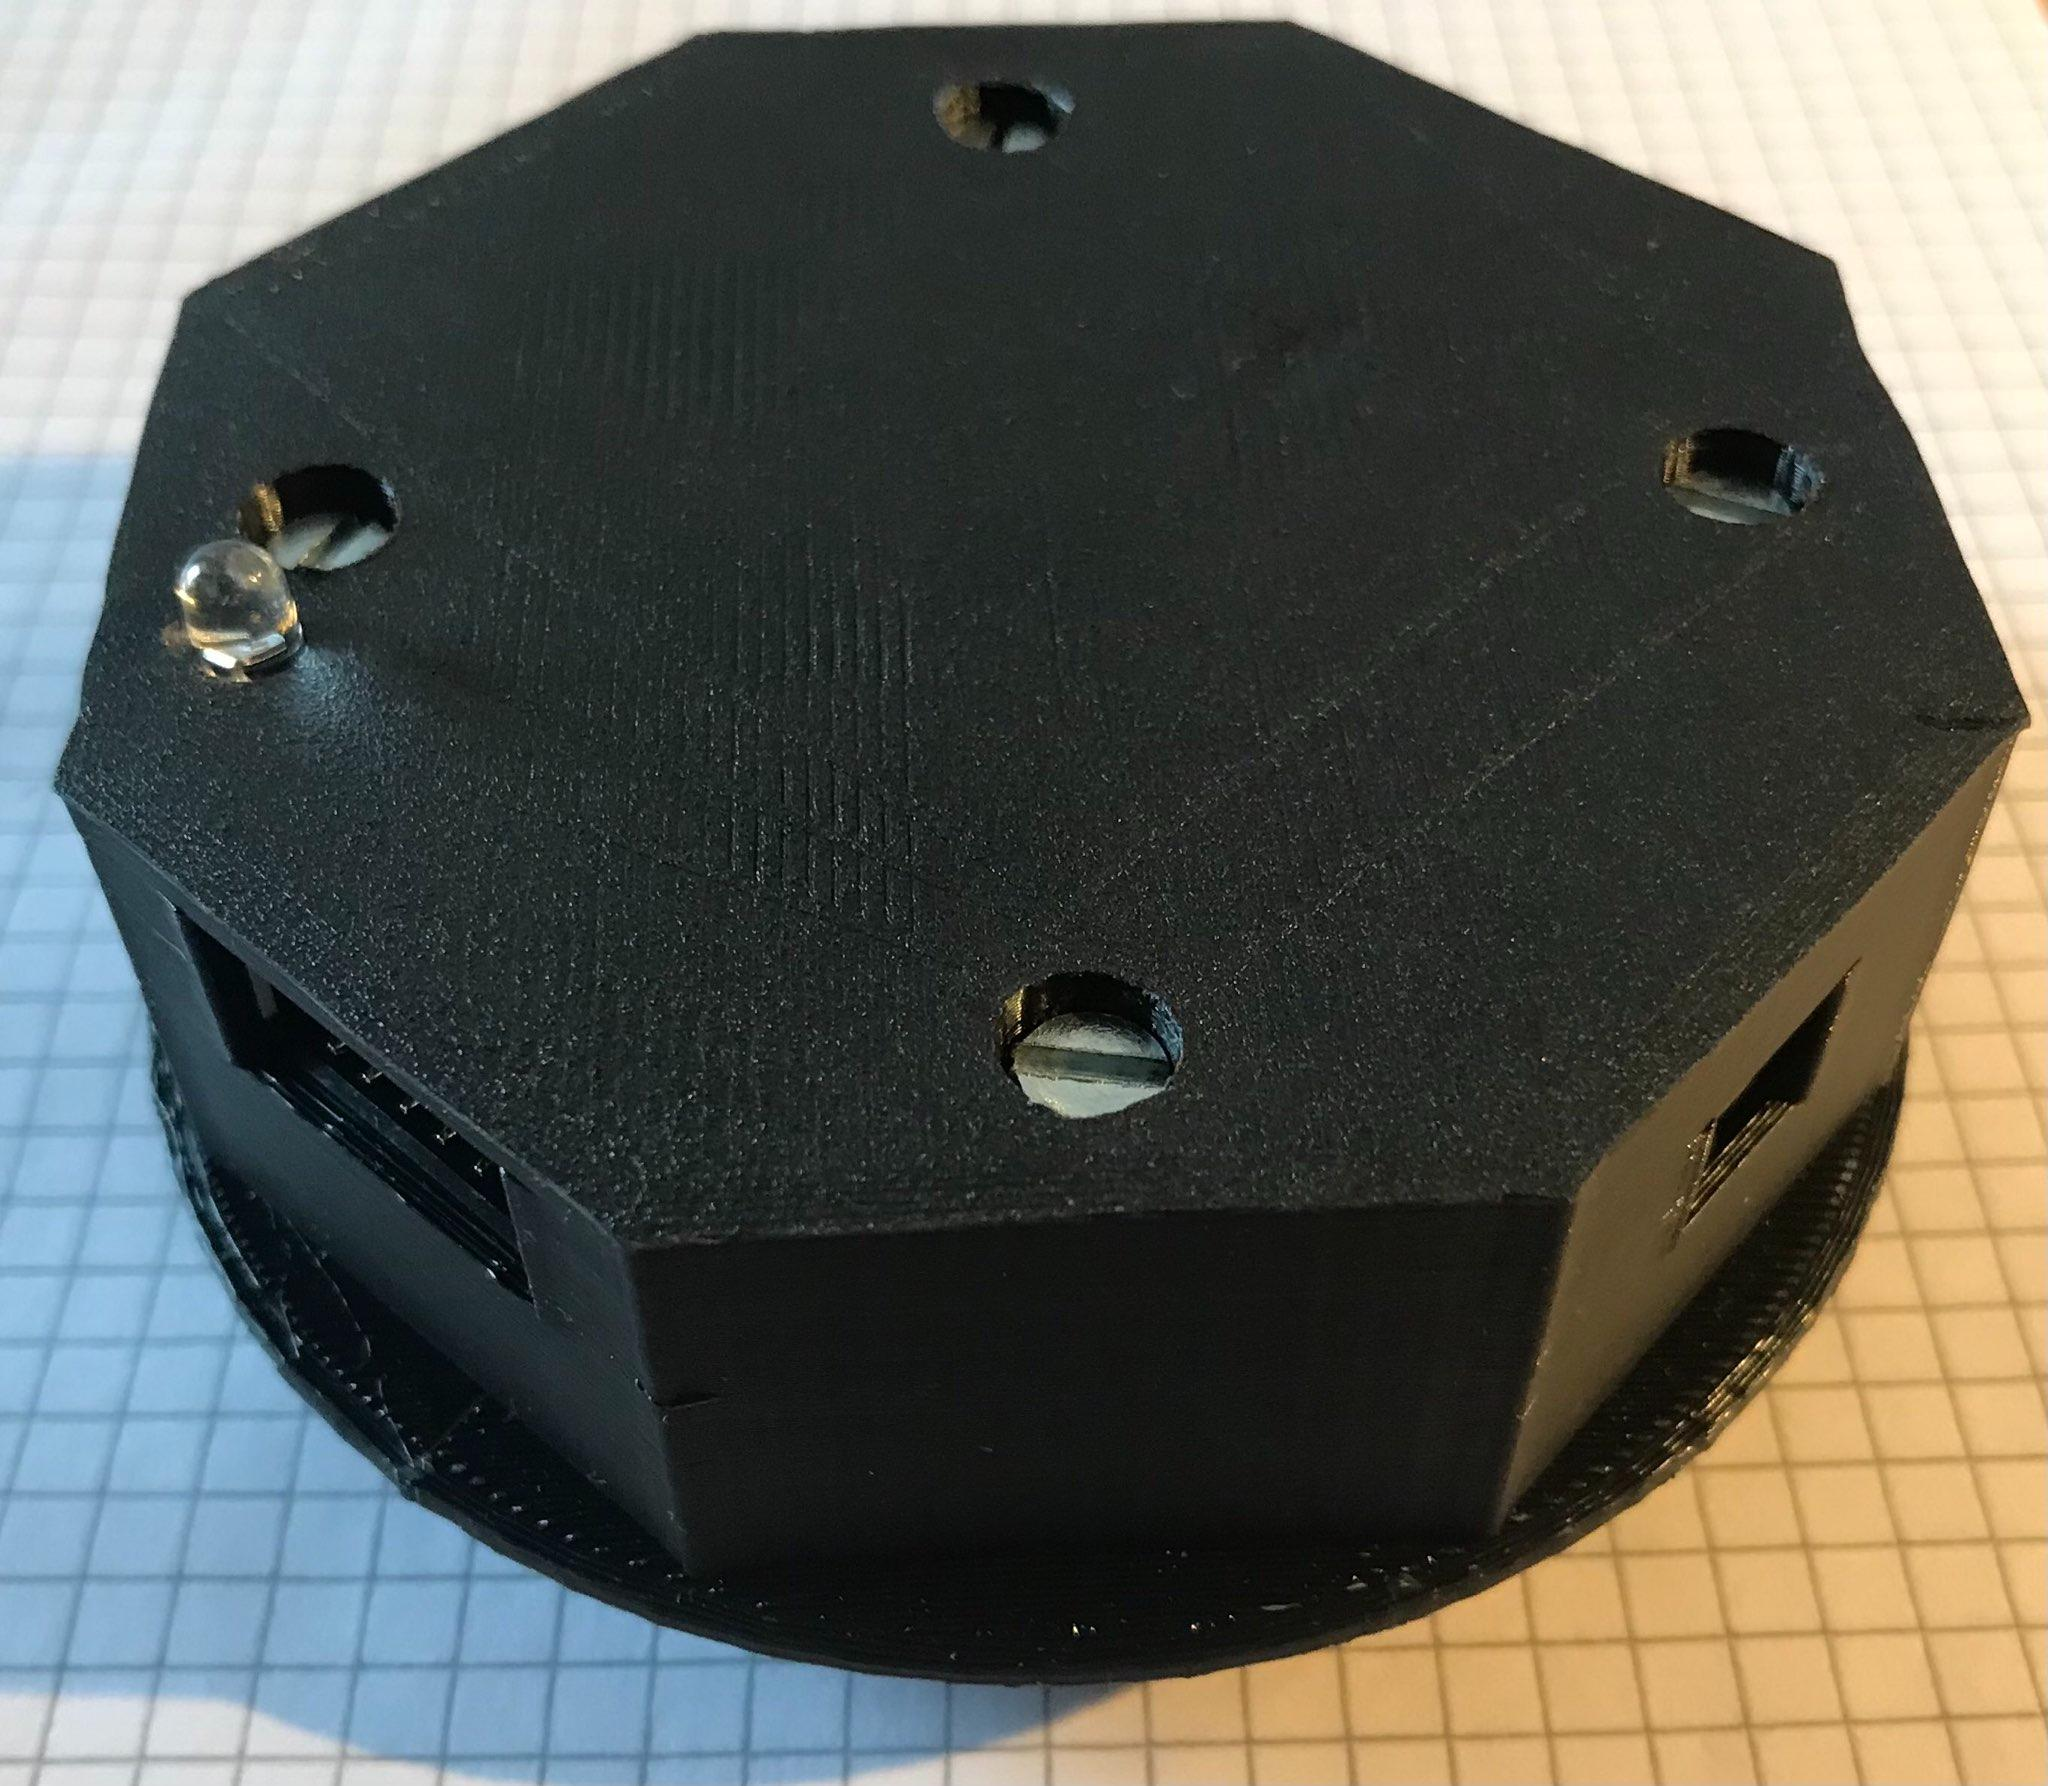
\includegraphics[width=0.7\textwidth]{pic/Komplett}
	\caption{Vollständig montiertes Gerät}
	\label{fig:Komplett}
\end{figure}

\chapter{Elektronik}
\label{ch:elektronik}
Die Elektronik besteht aus der Hauptplatine, die in fünf Funktionsblöcke unterteilt ist, einer Adapterplatine für den Luftsensor und einem ansteckbaren Bodenfeuchtigkeitssensor. Die Funktionsblöcke ensprechen den Seiten von "`biosphereMonitor.sch"', die Adapterplatine findet sich in "`Adapter.sch"'. Beide Schaltpläne und ihre dazugehörigen Platinen sind mit Eagle verfasst worden.

Eagle ist in als Demoversion und für Bildungszwecke kostenlos und lässt sich unter \url{https://www.autodesk.de/products/eagle/free-download}\\ herunterladen.
\section{Mikrocontroller}
\label{sec:Mikrocontroller}
Alls Mikroncontroller findet ein ATxmega32A4AU\cite{ds:xmega} oder 16A4AU von Microchip Verwendung (IC1). Dieser wird über die PDI Schnittstelle auf JP2 Programmiert. Das Pinout dieses Steckers ist kompaktibel mit dem des AVR ISP MK II Programiergeräts von Atmel/Microchip.

An Pin 36 und 37 ist der Hauptquartz Q1 angeschlossen. Die Frequenz dieses Quartzes kann 4 bis 20MHz betragen und muss in "`main.c"' und "`makefile"' als F\_CPU eingetragen werden. Standard ist 16MHz.

An Pin 32 und 33 ist Q2, der 32,768kHz Uhrenquartz für die Realtimeclock angebracht.

Pin 42 und 43 sind analoge Eingänge für Temperatursensor (siehe \autoref{sec:Außensensoren}) und Bodenfeuchtigkeitssensor (siehe \autoref{sec:Bodenfeuchtigkeitssensor}), Pin 40 die Analoge Referenzspannung. Diese wird mit einem 33k/22k Spannungsteiler von 2,5V auf 1V geteilt.

Pin 12 (Tx) und 13 (Rx) verbinden UART0 mit dem USB UART Wandler (\autoref{sec:USB-UART Wandler}). In Revision 1.0 der Platinen sind diese Pins vertauscht, weshalb sie mit angelöteten Drähten vertauscht werden müssen.

Pin 26 und 27 sind die eingebaute USB Schnittstelle. Diese wird aktuell nicht genutzt, es ist jedoch eine Verbindung zum USB Stecker JP1 vorgesehen.

Pin 25 ist der Eingang vom Lichtsensor (\autoref{sec:Außensensoren}) und löst intern bei Steigender Flanke einen Pin Change Interuppt aus.

Pin 10 und 11 sind mit TWI C, der I²C Schnittstelle für den Luftsensoren (\autoref{sec:Adapterplatine}) belegt.

Pin 14 bis 17 sind mit der Spi Schnittstelle, Pin 20 und 21 mit den Kontrollsignalen für den Spi Flash belegt.
Bei diesem Flash handelt es sich um einen 4Mb 

\begin{figure}[h]
	\centering
	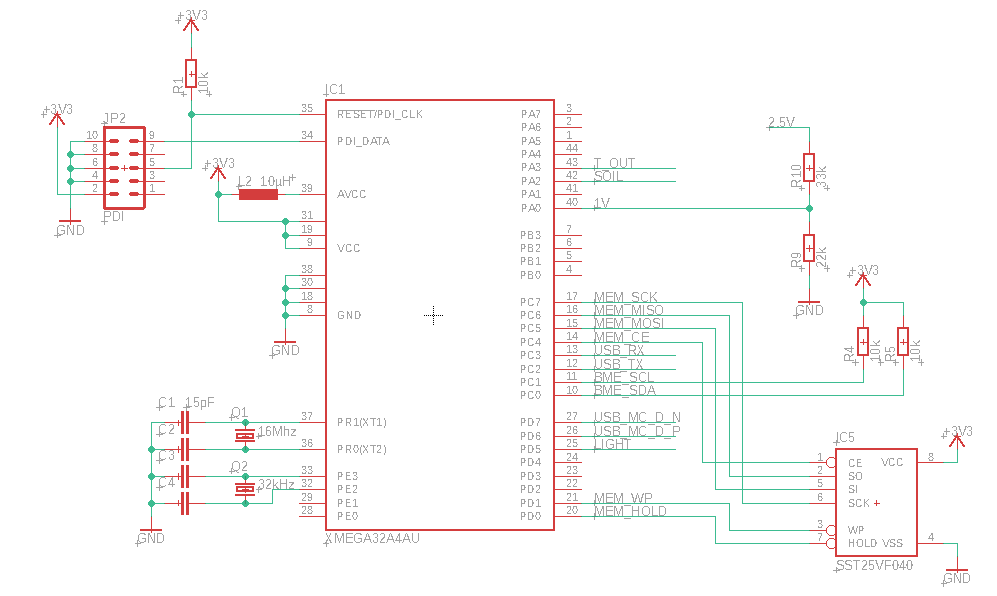
\includegraphics[width=1\textwidth]{pic/Microcontroller}
	\caption{Schaltplan Mikrocontroller}
	\label{fig:Microcontroller}
\end{figure}

\section{Stromverteilung}
\label{sec:Stromverteilung}

\section{USB-UART Wandler}
\label{sec:USB-UART Wandler}

\section{Außensensoren}
\label{sec:Außensensoren}

\section{Anschlüsse Innensensoren}
\label{sec:Innensensoren}

\section{Adapterplatine}
\label{sec:Adapterplatine}

\section{Bodenfeuchtigkeitssensor}
\label{sec:Bodenfeuchtigkeitssensor}

\begin{thebibliography}{9}
\raggedright 

\bibitem{Github}
  Tjark Gaudich,
  \textit{Biospher Monitor},\\
  \url{github.com/TjarkG/biosphere-monitor}\\
  GitHub.com,
  2021
  
\bibitem{Tafelwerk}
  Prof.~Dr.~Lothar Meyer et al.,
  \textit{Das große Tafelwerk interaktiv 2.0},
  Cornelsen Verlag, Berlin,
  1. Auflage, 8. Druck 2018
  
\bibitem{ds:xmega}
  Microchip Technology Inc.,
  \textit{ATxmega32A4U datasheet},\\
  \url{www.microchip.com/downloads/en/DeviceDoc/ATxmega128-64-32-16A4U-DataSheet-DS40002166A.pdf}\\
  Microchip.com,
  2011-2020
  
\bibitem{ds:Flash}
  Microchip Technology Inc.,
  \textit{SST25VF040 datasheet},\\
  \url{www.microchip.com/downloads/en/DeviceDoc/20005051E.pdf}\\
  Microchip.com,
  2005-2020
  
\bibitem{ds:usb}
  Future Technology Devices International Limited,
  \textit{FT2323R datasheet},\\
  \url{www.ftdichip.com/wp-content/uploads/2020/08/DS_FT232R.pdf}\\
  ftdichip.com, 2020
  
\bibitem{ds:temp}
  Texas Instruments Incorporated,
  \textit{LM35 datasheet},\\
  \url{www.ti.com/lit/gpn/lm35}\\
  TI.com,
  1999-2017
  
\bibitem{ds:light}
  Vishay Semiconductors,
  \textit{BPW96 datasheet},\\
  \url{www.vishay.com/docs/81532/bpw96.pdf}\\
  vishay.com,
  2011
  
\bibitem{ds:BMP280}
  Bosch Sensortec GmbH,
  \textit{BMP280 datasheet},\\
  \url{www.bosch-sensortec.com/media/boschsensortec/downloads/datasheets/bst-bmp280-ds001.pdf}\\
  bosch-sensortec.com,
  Oktober 2021
  
\bibitem{ds:BME280}
  Bosch Sensortec GmbH,
  \textit{BME280 datasheet},\\
  \url{www.bosch-sensortec.com/media/boschsensortec/downloads/datasheets/bst-bme280-ds002.pdf}\\
  bosch-sensortec.com,
  Oktober 2021
  
\bibitem{ds:BME680}
  Bosch Sensortec GmbH,
  \textit{BME680 datasheet},\\
  \url{www.bosch-sensortec.com/media/boschsensortec/downloads/datasheets/bst-bme680-ds001.pdf}\\
  bosch-sensortec.com,
  Januar 2021

\bibitem{CLanguage}
  Brian W.Kernighan, Dennis M.Ritchie,
  \textit{The C Programming Language},
  Prentice Hall PTR, New Jersey,
  2. Auflage, 58. Druck 2018

\end{thebibliography}

\end{document}